\documentclass[letterpaper]{exam}

\usepackage[margin=1in, top=0.7in]{geometry}
\usepackage{tikz}

\tikzstyle{block} = [rectangle, draw, text centered, minimum width = 3em, minimum height = 3em]

\begin{document}

\begin{center}
	\textbf{CS 482 - Rich Internet Applications} \\
	\textbf{Section 801} \\
	\textbf{Quiz 3} \\
	\vspace{5mm}
	\makebox[\textwidth]{Name :\enspace\hrulefill} \\
\end{center}


\begin{questions}
	\question[5] This image file \texttt{dice.jpg} is 120 x 80 pixels in size. It is composed of 6 40 x 40 sub-images.
		\begin{figure}[ht!]
			\centering
			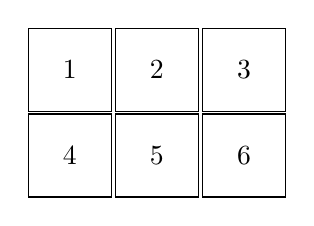
\begin{tikzpicture}
				\node[block] (1) {1};
				\node[block, right of=1, node distance=3.15em] (2) {2};
				\node[block, right of=2, node distance=3.15em] (3) {3};
				\node[block, below of=1, node distance=3.1em] (4) {4};
				\node[block, right of=4, node distance=3.15em] (5) {5};
				\node[block, right of=5, node distance=3.15em] (6) {6};
			\end{tikzpicture}
		\end{figure}
	\\
		A 40 x 40 \texttt{div} (\texttt{id="this"}) has been assigned this image as its background-image. Write \texttt{CSS} code that will cause just the \texttt{5} to be displayed.
	\vspace{\stretch{1}}
	
	\question[5] Write a function that returns a random integer from 1 to 6.
	\vspace{\stretch{1}}
		
\end{questions}


\end{document}